%----------------------------------------------------------------------------------------
%	PACKAGES AND OTHER DOCUMENT CONFIGURATIONS
%----------------------------------------------------------------------------------------
\documentclass[paper=a4, fontsize=11pt]{scrartcl} % A4 paper and 11pt font size
\usepackage[T1]{fontenc} % Use 8-bit encoding that has 256 glyphs
\usepackage{fourier} % Use the Adobe Utopia font for the document - comment this line to return to the LaTeX default
\usepackage[english]{babel} % English language/hyphenation
\usepackage{amsmath,amsfonts,amsthm} % Math packages
\usepackage{lipsum} % Used for inserting dummy 'Lorem ipsum' text into the template
\usepackage{sectsty} % Allows customizing section commands
\allsectionsfont{\centering \normalfont\scshape} % Make all sections centered, the default font and small caps
\usepackage{fancyhdr} % Custom headers and footers
\usepackage{amsmath}
\usepackage{graphics}
\usepackage{graphicx}

\pagestyle{fancyplain} % Makes all pages in the document conform to the custom headers and footers
\fancyhead{} % No page header - if you want one, create it in the same way as the footers below
\fancyfoot[L]{} % Empty left footer
\fancyfoot[C]{} % Empty center footer
\fancyfoot[R]{\thepage} % Page numbering for right footer
\renewcommand{\headrulewidth}{0pt} % Remove header underlines
\renewcommand{\footrulewidth}{0pt} % Remove footer underlines
\setlength{\headheight}{13.6pt} % Customize the height of the header

\numberwithin{equation}{section} % Number equations within sections (i.e. 1.1, 1.2, 2.1, 2.2 instead of 1, 2, 3, 4)
\numberwithin{figure}{section} % Number figures within sections (i.e. 1.1, 1.2, 2.1, 2.2 instead of 1, 2, 3, 4)
\numberwithin{table}{section} % Number tables within sections (i.e. 1.1, 1.2, 2.1, 2.2 instead of 1, 2, 3, 4)

\setlength\parindent{0pt} % Removes all indentation from paragraphs - comment this line for an assignment with lots of text

%----------------------------------------------------------------------------------------
%	TITLE SECTION
%----------------------------------------------------------------------------------------

\newcommand{\horrule}[1]{\rule{\linewidth}{#1}} % Create horizontal rule command with 1 argument of height

\title{	
\normalfont \normalsize 
\horrule{0.5pt} \\[0.4cm] % Thin top horizontal rule
\huge CS 760 Homework 3: Neural Network\\ % The assignment title
\horrule{2pt} \\[0.5cm] % Thick bottom horizontal rule
}

\author{Qihong Lu} % Your name
\date{\normalsize\today} % Today's date or a custom date

\begin{document}

\maketitle % Print the title

%----------------------------------------------------------------------------------------
%	PROBLEM 1
%----------------------------------------------------------------------------------------

\section*{Question1}

To run the program, type the following command: 
$$ \text{./nnet l h e <train-set-file> <test-set-file>} $$ 
where l specifies the learning rate, h the number of hidden units and e the number of training epochs. \\\\\\

Code: 
\begin{itemize}
	\item nn\_alg.py: implements binary classification network with zero or one hidden layer 
	\item util.py: the definitions of some constants and helper functions 
	\item nnet.py: run neural network, return test results
\end{itemize}
 
\hfill 

Dependencies: 
\begin{itemize}
  \item pyhton 2.7 
  \item numpy 
  \item scipy 
  \item sys
\end{itemize}



%----------------------------------------------------------------------------------------
%	PROBLEM 2
%----------------------------------------------------------------------------------------
\newpage
\section*{Question2}
\textbf{Using heart\_train.arff and heart\_test.arff, you should make two graphs showing error-rates versus the number of training epochs. For the first graph, plot training and testing error rates for a single-layer network trained for 1, 10, 100 and 500 epochs, using a learning rate of 0.1. For the second graph, plot similar curves for a network with 20 hidden units. }
\begin{center}
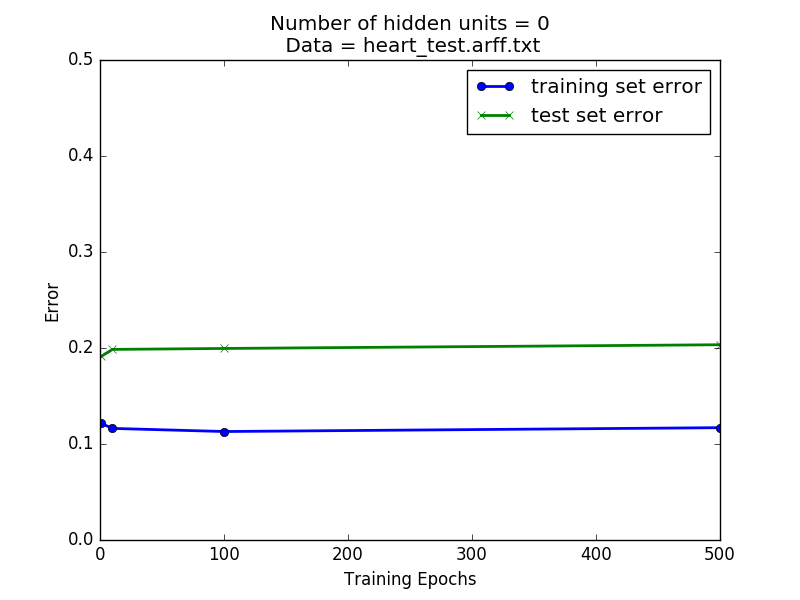
\includegraphics[scale=.45]{pics/learningCurve_noHidden.png}
\end{center}
\begin{center}
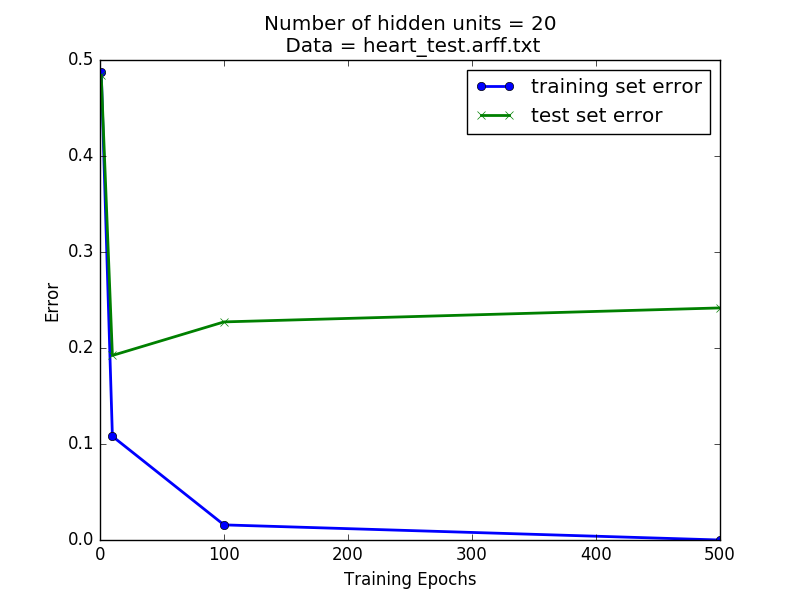
\includegraphics[scale=.45]{pics/learningCurve_hidden.png}
\end{center}

The learning curves above are the average results of 20 runs. Although the model with hidden units (the bottom figure) did better at reducing the training error, but its test error is higher, compared to the simpler perceptron (without hidden layer). This suggests that the model with 20 hidden units is overfitting the training set. This issue of overfitting (the bottom figure) can also be seen from the increasing trend of the test error over the training epochs. 


%----------------------------------------------------------------------------------------
%	PROBLEM 3
%----------------------------------------------------------------------------------------
\newpage
\section*{Question3}
\textbf{For this part, you should produce ROC curves for two data sets. Use the activation of the output unit as the measure of confidence that a given test instance is positive, and plot ROC curves for both the heart data set indicated above, and the lymphography data set lymph\_train.arff, lymph\_test.arff. Be sure to label the axes of your plots.}

\begin{center}
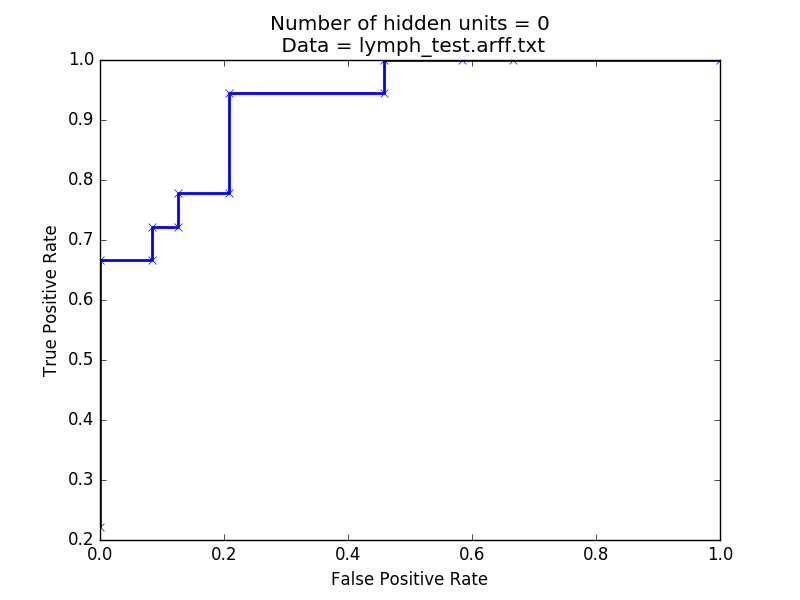
\includegraphics[scale=.5]{pics/roc_noHidden.png}
\end{center}

\begin{center}
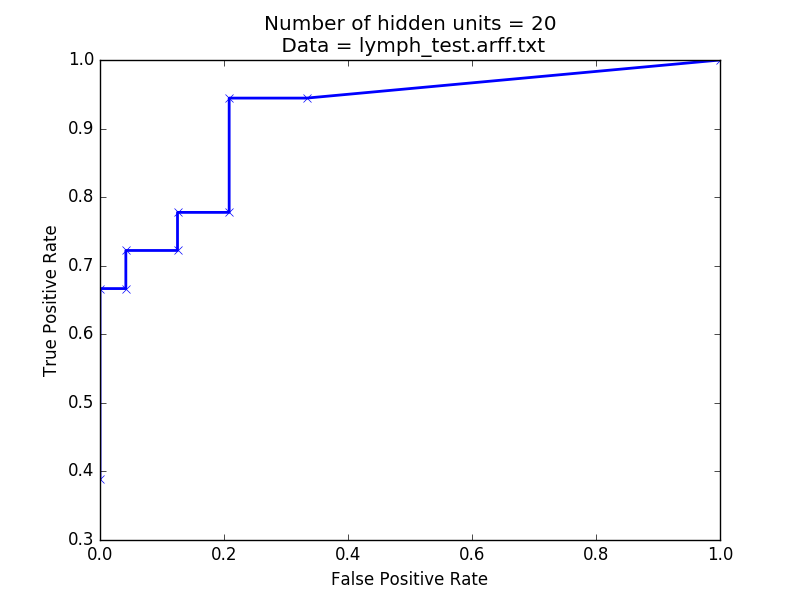
\includegraphics[scale=.5]{pics/roc_hidden.png}
\end{center}

In this simulation, both models were trained for 500 epochs with learning rate of .1. The model with the hidden layer has five hidden units. It turned out that the model with five hidden units achieved a better accuracy, suggesting the simple perceptron is slightly underfitting the data. 

\end{document}